%%%%%%%%%%%%%%%%%%%%%%%%%%%%%%%%%%%%%%%%%%%%%%%%%%%%%%%%%%%%%%%%%%%%%%%%%%%%%%%%
%2345678901234567890123456789012345678901234567890123456789012345678901234567890
%        1         2         3         4         5         6         7         8

\documentclass[letterpaper, 10 pt, conference]{ieeeconf}  % Comment this line out if you need a4paper

%\documentclass[a4paper, 10pt, conference]{ieeeconf}      % Use this line for a4 paper

\IEEEoverridecommandlockouts                              % This command is only needed if 
                                                          % you want to use the \thanks command

\overrideIEEEmargins                                      % Needed to meet printer requirements.

%In case you encounter the following error:
%Error 1010 The PDF file may be corrupt (unable to OPEN PDF file) OR
%Error 1000 An error occurred while parsing a contents stream. Unable to analyze the PDF file.
%This is a known problem with pdfLaTeX conversion filter. The file cannot be OPENed with acrobat reader
%Please use one of the alternatives below to circumvent this error by uncommenting one or the other
%\pdfobjcompresslevel=0
%\pdfminorversion=4

% See the \addtolength command later in the file to balance the column lengths
% on the last page of the document

\usepackage[bookmarks=true]{hyperref}
\usepackage{graphicx}
\usepackage[font=footnotesize]{subcaption}
\usepackage[font=footnotesize]{caption}
\usepackage{hyperref}
\usepackage{url}
\usepackage{amsmath,amssymb,amsfonts,amsfonts}
% \usepackage{algorithm}
% \usepackage[noend]{algorithmic}
\usepackage{xspace}
\usepackage{wrapfig}
\usepackage{color}

\usepackage{algorithm}
\usepackage{algorithmicx}
\usepackage[noend]{algpseudocode}
\usepackage{algpseudocode}
\algrenewcommand\algorithmicindent{1.0em}%


\newcommand{\calX}{\ensuremath{\mathcal{X}}\xspace}
\newcommand{\calL}{\ensuremath{\mathcal{L}}\xspace}
\newcommand{\calS}{\ensuremath{\mathcal{S}}\xspace}
\newcommand{\calR}{\ensuremath{\mathcal{R}}\xspace}

\newcommand{\sAttract}{\ensuremath{s^{\text{attractor}}_i}\xspace}
\newcommand{\sStart}{\ensuremath{s_{\text{start}}\xspace}}
\newcommand{\sGoal}{\ensuremath{s_{\text{goal}}\xspace}}
\newcommand{\sNom}{\ensuremath{s_{\text{nominal}}\xspace}}


\title{\LARGE \bf
Provable Infinite-Horizon Real-Time Planning for Repetitive Tasks
}


% \author{Albert Author$^{1}$ and Bernard D. Researcher$^{2}$% <-this % stops a space
% \thanks{*This work was not supported by any organization}% <-this % stops a space
% \thanks{$^{1}$Albert Author is with Faculty of Electrical Engineering, Mathematics and Computer Science,
%         University of Twente, 7500 AE Enschede, The Netherlands
%         {\tt\small albert.author@papercept.net}}%
% \thanks{$^{2}$Bernard D. Researcheris with the Department of Electrical Engineering, Wright State University,
%         Dayton, OH 45435, USA
%         {\tt\small b.d.researcher@ieee.org}}%
% }

\author{
Fahad Islam,
Oren Salzman {\normalfont and}
Maxim Likhachev
\\
The Robotics Institute, Carnegie Mellon University\\
%
\{fi,osalzman\}@andrew.cmu.edu,
maxim@cs.cmu.edu
}

\begin{document}



\maketitle
\thispagestyle{empty}
\pagestyle{empty}


%%%%%%%%%%%%%%%%%%%%%%%%%%%%%%%%%%%%%%%%%%%%%%%%%%%%%%%%%%%%%%%%%%%%%%%%%%%%%%%%
\begin{abstract}

We consider the problem of solving high-dimensional motion-planning tasks in real-time for highly-repetitive tasks. 
Preprocessing-based approaches prove to be very beneficial in such settings---they analyze the state-space offline to generate some auxiliary information which can then be used in the query phase to speedup planning times. 
%
Typically, the tighter the requirement is on query times the larger the memory footprint will be. In particular, for high-dimensional spaces, providing real-time planning capabilities is impractical.
Moreover, as far as we are aware of, non of the general-purpose algorithms come with \emph{provable} guarantees on the maximal query time.
We propose a preprocessing-based method that provides provable bounds on the query time while incurring only a small amount of memory overhead in the query phase. We evaluate our method on a 7-DOF robot arm and show a speedup of over tenfold in query time when compared to the \textsf{PRM} algorithm while guaranteeing a maximum query time of less than {\color{blue} XXX} miliseconds.

\end{abstract}

%%%%%%%%%%%%%%%%%%%%%%%%%%%%%%%%%%%%%%%%%%%%%%%%%%%%%%%%%%%%%%%%%%%%%%%%%%%%%%%%
\section{Introduction}

%1. What is the problem?
Consider the problem of a robot picking up objects from a high-speed conveyor belt and placing them into bins (see Fig.~\ref{fig:PR2}).
Similarly, consider a robot given the task of stock replenishment---moving in a supermarket and loading items from a cart it carries to half-empty shelves.
%2. Why is it relevant?
These problems are examples of repetitive tasks performed by (possibly highly articulated) robots in static environments where the start and target of each repetitive task is similar, yet not identical, to previous tasks.
Difference in the exact start and target position may be due to uncertainty in the environment (objects placed on different parts of the conveyor belt or in different orientation) or due to highly-similar tasks (objects placed in similar positions on a shelf).

%3. Why is it hard?
As the set of possible start and target locations may be large, caching pre-computed paths for all these queries in advance is unmanageable. 
Clearly, once a task is presented to the robot, it can compute a desired path online.
However, this may incur large online planning times that may be unacceptable in many settings.
For example, in our conveyor-belt setting, reducing the planning time immediately corresponds to faster unloading capabilities. 
Moreover, if the planner cannot \emph{guarantee} to pick items from the conveyor in a timely manner, the system is required to account for missed items by e.g., additional conveyor belts that will redirect items back to the robot---a costly backup in terms of both time and space.
Thus, a natural approach is to preprocess the environment in an offline phase to allow for fast planning times online.

%4. What have others done?
One way to preprocess the environment is using the \textsf{PRM} algorithm~\cite{kavraki1996probabilistic}.
Once a a dense roadmap has been pre-computed, any query can be efficiently answered online by connecting the source and target to the roadmap. 
Query times can be significantly sped up by further preprocessing the roadmaps using landmarks~\cite{paden2017landmark}.
Unfortunately, there is no guarantee that a query can be connected to the roadmap as \textsf{PRM} only provides \emph{asymptotic} guarantees~\cite{KKL98}.
Furthermore, this connecting phase requires running a collision-detection algorithm which is typically considered the computational bottleneck in many motion-planning algorithms~\cite{L06}.

Recently, Lehner and  Albu{-}Sch{\"{a}}ffer~\cite{LA18} suggest the repetition roadmap to extend the \textsf{PRM} for the case of multiple highly-similar scenarios.
While their approach exhibits significant speedup in computation time, it still suffers from the previously-mentioned shortcomings.

A complementary approach to aggressively preprocess a given scenario is by minimizing collision-detection time.
However this requires designing robot-specific
circuitry~\cite{MFQSK16}
or limiting the approach to standard manipulators~\cite{YMILV18}.

An alternative approach is to precompute a set of complete paths into a library and given a query, attempt to match complete paths
from the library to the new query~\cite{berenson2012robot, jetchev2013fast}.
Unfortunately, this approach also cannot provide any of the guarantees required by our applications.

Our work bares resemblance to previous work on 
subgoal graphs~\cite{UK17,UK18} and to real-time planning~\cite{KL06,KS09,K90}.
However, in the former, the entire configuration space is preprocessed in order to efficiently answer queries between \emph{any} pair of states which deems it applicable only to low-dimensional spaces.
Similarly, in the latter, to provided guarantees on planning time the search only looks at a finite horizon and interleaves planning and execution.

\begin{figure}[tb]
  \centering
    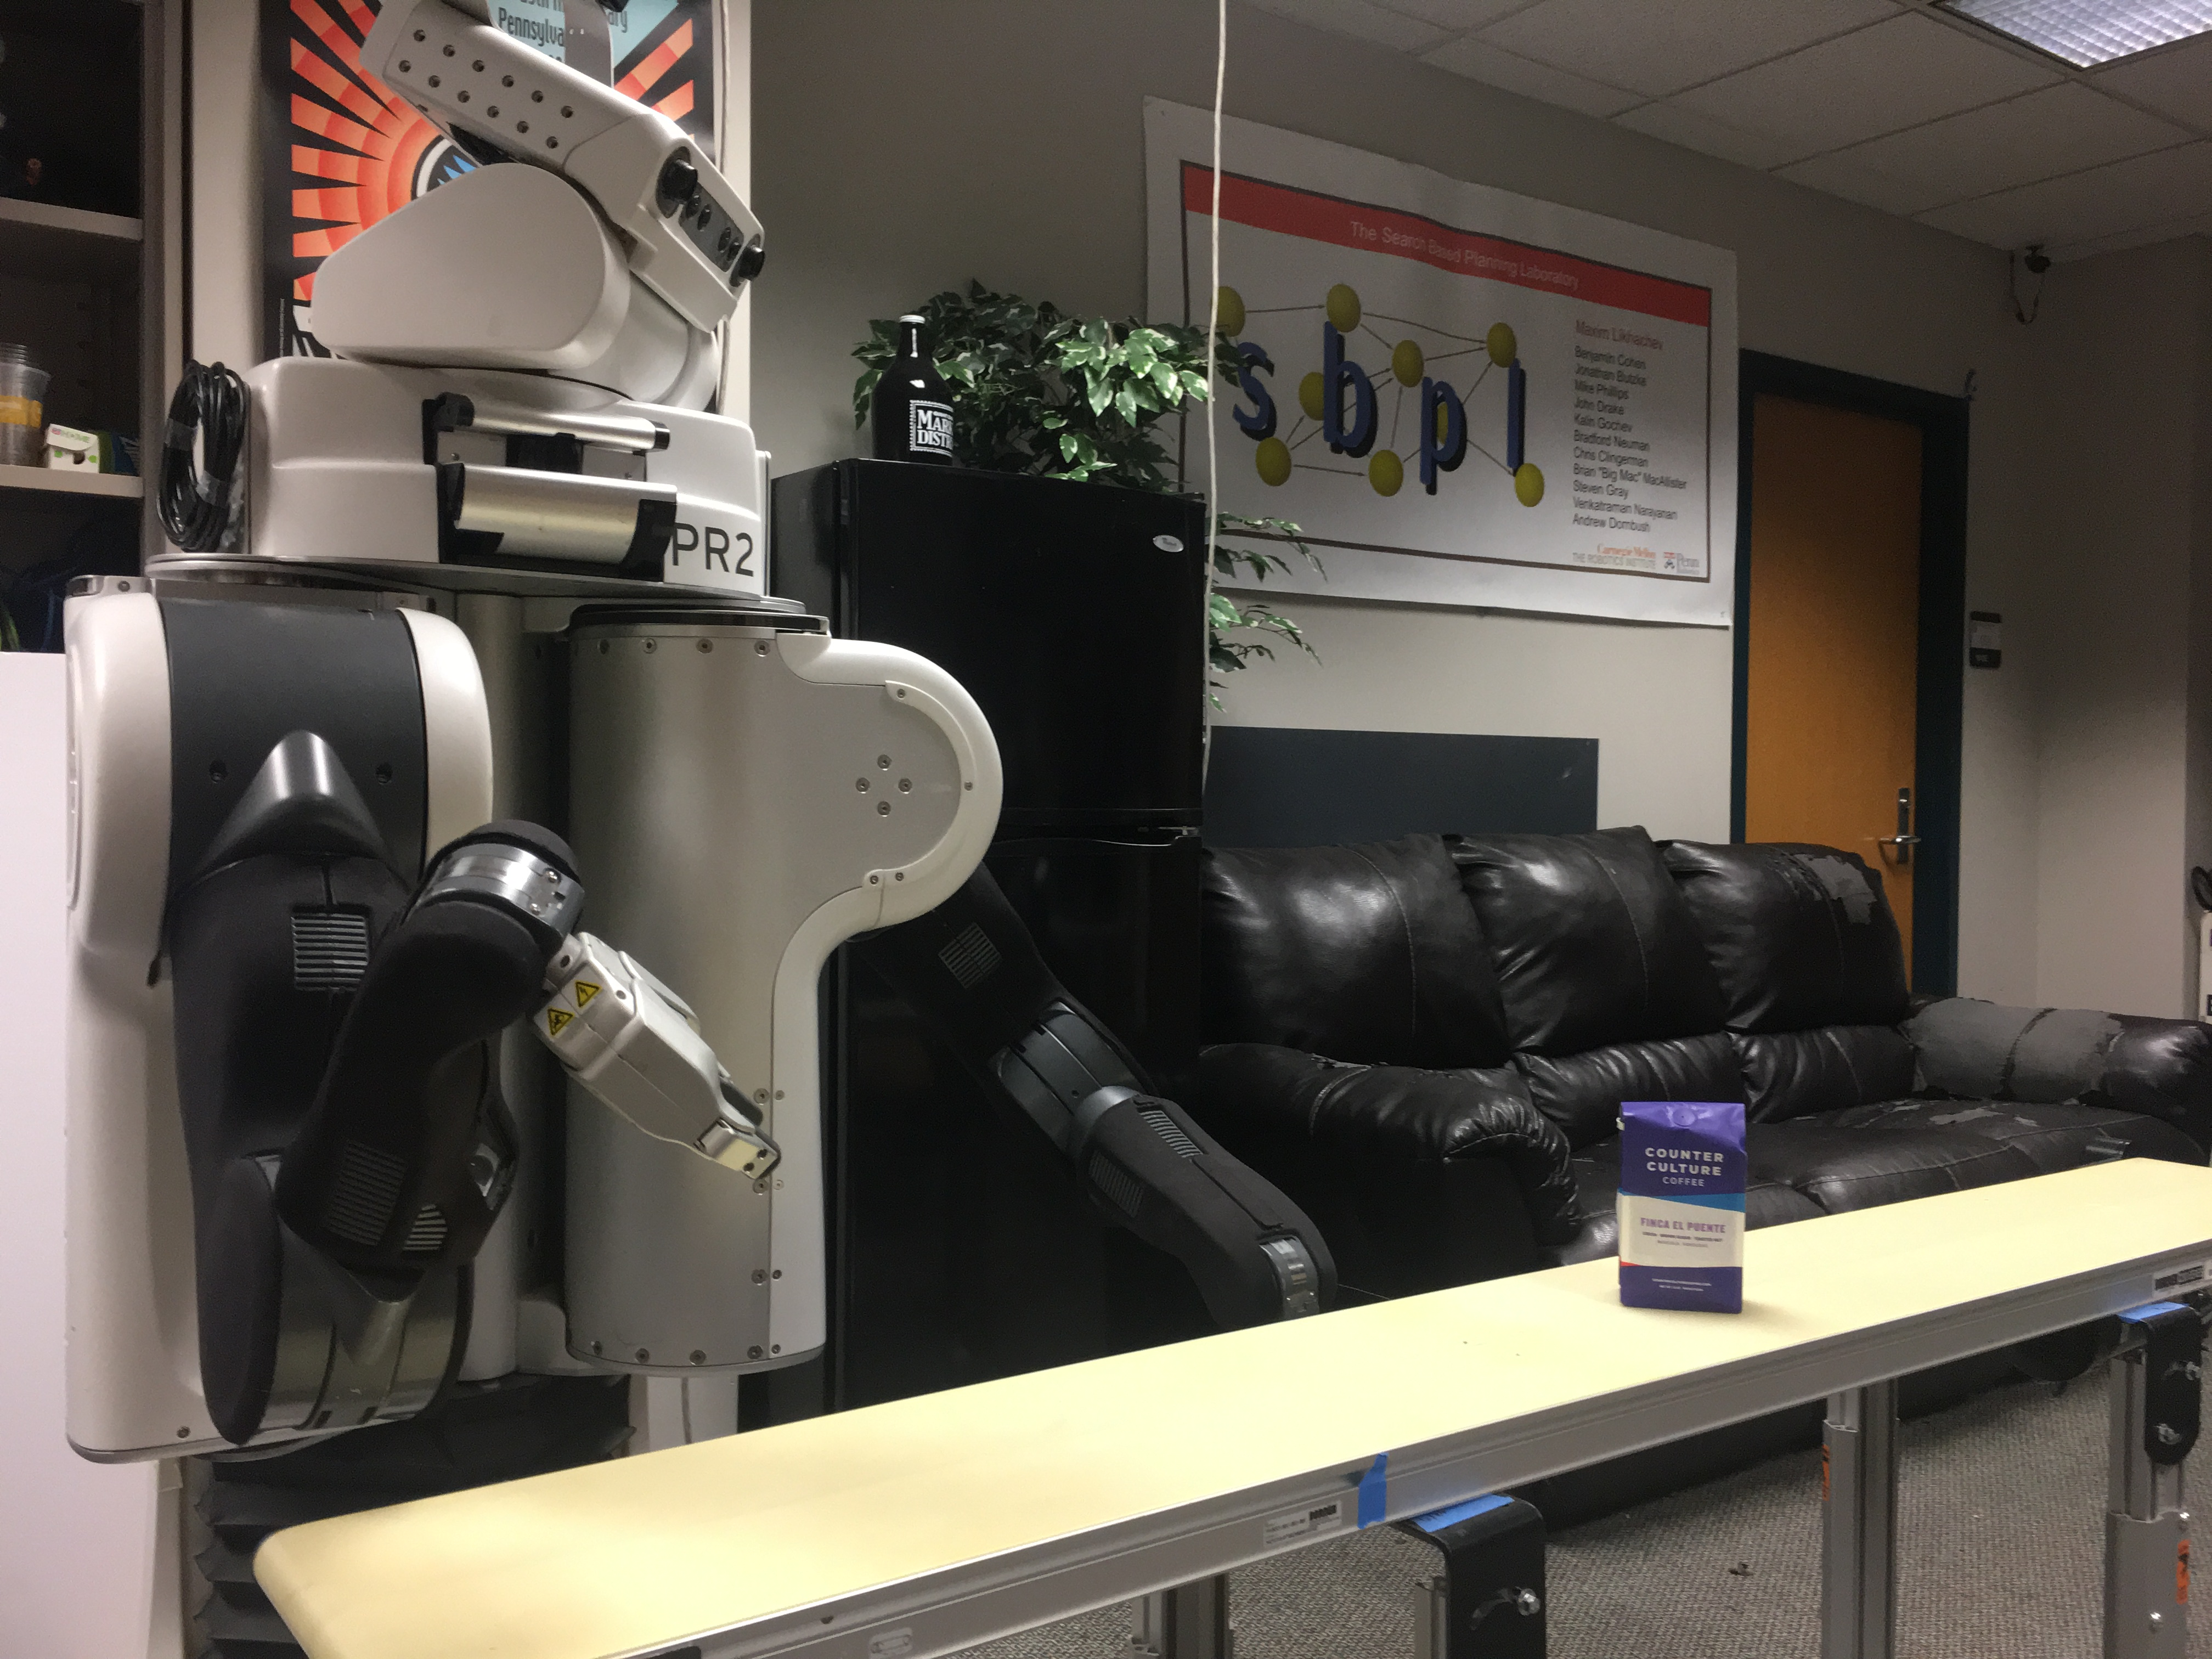
\includegraphics[width=0.25\textwidth]{PR2.jpg}
    % \vspace{-2mm}
  \caption{
  Motivating scenario---a robot (PR2) picking up objects from a conveyor belt.
}
    \label{fig:PR2}
 \vspace{-6mm}
\end{figure}

%5. What's missing?

%6. What is our ONE key insight?
Our key insight is to combine a precomputed library~$\calL$ of paths between \emph{several} start and target configurations together with a method to connect \emph{any} start and target configuration to a path in~$\calL$ \emph{without} having to perform collision detection.
This insight allows us to provide \emph{provable bounds} on the time to solve motion-planning queries which are in the order of milliseconds for a seven DOF manipulator.

%7. How do we compare against the state of the art?
We evaluate our approach in simulation on the PR2 robot\footnote{http://www.willowgarage.com/pages/pr2/overview} (see Fig.~\ref{fig:PR2} and~\ref{fig:sim})
and demonstrate a speedup of over tenfold in query time when compared to the \textsf{PRM} algorithm with little memory footprint and while guaranteeing a maximal query time of less than {\color{blue} XXX} miliseconds.

%8. What are our contributions?
%9. What are our limitations?

\section{Algorithm Framework}
%In this section we describe our algorithmic framework. We start (Sec.~\ref{sec:pdef}) by formally defining our problem and continue...
\subsection{Problem Formulation and assumptions}
Let $\calX$ be the configuration space of a robot operating in a static environment.
We are given in advance a start configuration~$\sStart \in \calX$ and some goal region~$G \subset \calX$.
In the query phase we are given multiple queries $(\sStart, s_{\text{goal}})$ where $s_{\rm goal} \in G$ and for each query, we need to compute a collision-free path connecting $\sStart$ to $s_{\text{goal}}$.

We discretize $\calX$ into a state lattice $\calS$ such that any state~$s \in \calS$ is connected to a set of successors via a mapping Succs: $\calS \rightarrow 2^\calS$ and make the following assumptions:

\begin{enumerate}
  \item[A1] The goal region~$G \subset \calX$ is a relatively small subset of the full configuration space of the robot. Namely, it is feasible to exhaustively iterate over all states in $G$.
However, storing a path from $\sStart$ to each state in $G$ is infeasible.
  
  \item[A2] The planner has access to a $\textit{weakly-monotonic}$ heuristic function $h: \calS \times \calS \rightarrow \mathbb{R}$ such that $\forall s_1, s_2  \in G$ where $s_1 \neq s_2$ it holds that,

  \begin{center}
    $h(s_1, s_2) \geq \min\limits_{\forall s_1' \in \text{Succs}(s_1)} h(s_1', s_2) \quad \forall s_1'\in G $. 
  \end{center}
  Namely, for any distinct pair of states ($s_1, s_2$) in $G$, at least one of $s_1$'s successors (also belonging to $G$) must have a heuristic value less than or equal to its heuristic value. 
	Note that this assumption does not imply  that~$G$ is collision free.
%	
%	
%  This property should hold assuming that all the edges in $G$ are traversable i.e., they have finite costs.
%  {\color{blue} I don't understand the last sentence}
  % $G$ is defined as a 6-dimensional window around some nominal goal pose in the task space, $q = (\textit{x, y, z, roll, pitch, yaw})$.
\end{enumerate}

These assumptions allow us to establish strong theoretical properties regarding the efficiency of our planner. Namely, that
within a known bounded time, we can compute a collision-free path from $\sStart$ to any state in $G$. Proofs are omitted due to lack of space. 

\subsection{Key Idea}
Our planner comprises of a preprocessing and a query phase. 
In the preprocessing phase, $G$ is decomposed into a finite  set of (possibly overlapping) subregions $\calR$.
Each subregion $R_i \in \calR$ is a hyper-ball defined using a center which we refer to as the ``attractor state''~
\sAttract and a radius $r_i$.
% centered around what we call the $attractor$ states $s_{attractor_i}$ and radii $r_i$, where $i$ = 1 to $n$. 
These regions are constructed in such a way that the following two properties hold
\begin{enumerate}
  \item[P1] For any goal state $s_{\text{goal}} \in R_i \cap G$, a greedy search with respect to $h(s, \sAttract)$ over $\calS$ starting at $\sStart$ will result in a collision-free path to \sAttract.
  \item[P2] The union of all the subregions completely cover $G$. 
  		Namely, $\forall s \in \calS \cap G, \exists R_i \ s.t. \ s \in R_i$.
  		%In other words, any query state $\sGoal \in G$ will fall in atleast one of the subregions.
\end{enumerate}

In the preprocessing stage, we precompute a library of collision-free paths $\calL$ which includes one path from $\sStart$ to each attractor state. 
In the query phase, given a query~\sGoal, we 
(i)~identify a region $R_i$ such $\sGoal \in R_i$ (using the precomputed radii~$r_i$),
(ii)~run a greedy search towards~\sAttract by greedily choosing at every point the successor that minimizes~$h$ and
(iii)~append this path with the precomputed path in $\calL$ to $\sStart$ to obtain the complete plan.

\subsection {Algorithm}
\subsubsection{Preprocessing Phase}
The preprocessing phase of our algorithm, detailed in Alg.~\ref{alg:1}, takes as input the start state~$\sStart$ and the goal region~$G$ and outputs a set of subregions~$\calR$ and the corresponding library of paths~$\calL$ from each \sAttract to~\sStart. 

The algorithm covers~$G$ by iteratively finding a state $s$ not covered by any region and computing a new region centered at $s$.
To ensure that $G$ is complete covered (property P2) we maintain a set~$V$ of valid (collision free) and a set $I$ of invalid (in collision) states called \emph{frontier states} (lines~\ref{alg:1:v} and~\ref{alg:1:i}, respectively).
We start by initializing~$V$ to some random state in $G$ and iterate until both~$V$ and~$I$ are empty, which will ensure that $G$ is indeed covered.

At every iteration, we pop a state from $V$ (line~\ref{alg:1:pop}), and if there is no region covering it, we add it as a new attractor state and compute a path $\pi_i$ to $\sStart$ (line~\ref{alg:1:path}).
We then compute the corresponding region (line~\ref{alg:1:cr} and Alg.~\ref{alg:2}).

As we will see shortly, computing a region corresponds to a Dijkstra-like search centered at the attractor state.
The search terminates with the region's radius $r_i$ and a list of frontier states that comprise of the region's boundary.
The valid and invalid states are then added to $V$ and $I$, respectively (lines~\ref{alg:1:insert_v} and~\ref{alg:1:insert_i}).


Once $V$ gets empty the algorithm starts to search for states which are invalid and yet uncovered by growing regions around the states popped from~$I$ (lines~\ref{alg:1:iv_loop}-\ref{alg:1:iv_region}). If a valid and uncovered state is found, it is added to $V$ and the algorithm goes back to computing subregions (lines~\ref{alg:1:x_states}-\ref{alg:1:break}), otherwise if $I$ also gets empty, the algorithm terminates and it is guaranteed that each valid state contained in $G$ is covered under at least one subregion.

%{\color{blue} What is SearchValidUncoveredStates?.}


\begin{algorithm}[t]
\footnotesize
\hspace*{\algorithmicindent} \textbf{Inputs:} $G$, $\sStart$   
\Comment{goal region and start state} 

\hspace*{\algorithmicindent} \textbf{Outputs:} 
$\calR, \calL$
%$R_i = (\sAttract, r_i)$, $\pi_i$,
\Comment{subregions and corresponding paths to $\sStart$} 

%\hspace*{\algorithmicindent}
% \textbf{Parameters:} $r_{\text{max}}$   \Comment{maximum radius of a region}
\caption{Goal Region Preprocessing}\label{alg:1}


\begin{algorithmic}[1]
\Procedure{PreprocessRegion}{$G$}
%\Procedure{PreprocessRegion}{$G, r_{\text{max}}$}
  \State $s \leftarrow$\textsc{ SampleValidState}($G$)  
  \State $V \leftarrow \{ s \}$   \Comment{valid frontier states initialized to a random state} \label{alg:1:v}
  \State $I$ = $\emptyset$   \Comment{invalid frontier states} \label{alg:1:i}
  \State $ i \leftarrow 0$
  		 \hspace{2mm} 
  		 $\calL = \emptyset$
  		 \hspace{2mm} 
  		 $\calR = \emptyset$
  		 
  \vspace{2mm}
    \While {$V$ and $I$ are not empty}
        \While {$V$ is not empty}
          \State $s \leftarrow V.\text{pop}()$ \label{alg:1:pop}
            \If {$\nexists R \in \calR$  s.t. $s \in R$ }  \label{alg:1:discard}
            \Comment{$s$ is not covered}
				\State $\sAttract \leftarrow s$                
                \State $\pi_i$ = \textsc{PlanPath}($\sAttract , \sStart$);
                \hspace{2mm }
                $\calL \leftarrow \calL \cup \{ \pi_i \}$  \label{alg:1:path}
                \State $(\text{OPEN}, r_i) \leftarrow$ \textsc{ComputeReachability}($\sAttract$) \label{alg:1:cr}
%                \State $(\text{OPEN}, r_i) \leftarrow$ \textsc{ComputeReachability}($\sAttract, r_{\text{max}}$) \label{alg:1:cr}
                \State insert Valid(OPEN) in $V$  \label{alg:1:insert_v}
                \State insert Invalid(OPEN) in $I$   \label{alg:1:insert_i}
                \State $R_i$ $\leftarrow$ $(\sAttract, r_i)$; 
                \hspace{2mm} $ i \leftarrow i+1$				\hspace{2mm }
                $\calR \leftarrow \calR \cup \{ R_i \}$
                            \EndIf
        \EndWhile

\vspace{2mm}        
        
        \While {$I$ is not empty} \label{alg:1:iv_loop}
            \State $s$ $\leftarrow$ $I.pop()$
			\If {$\nexists R \in \calR$ s.t. $s \in R$ }      \Comment{$s$ is not covered}
\State $(X, r)$ $\leftarrow$ \textsc{SearchValidUncoveredStates}($s$)
%                \State $(X, r)$ $\leftarrow$ \textsc{SearchValidUncoveredStates}($s, r_{\text{max}}$)
                \State $\hat{R}_i$ $\leftarrow$ $(s,r)$;
				\hspace{2mm}
				$\calR \leftarrow \calR \cup \{ \hat{R}_i \}$ \Comment{invalid region}  \label{alg:1:iv_region}
                \If {$X$ is not empty}  \Comment{no valid state found}  \label{alg:1:x_states}
                    \State insert $X$ in $V$
                    \State \textbf{break} \label{alg:1:break}
                \EndIf
            \EndIf
        \EndWhile
    \EndWhile

  \vspace{2mm}

  \State \Return $\calR, \calL$
\EndProcedure
\end{algorithmic}
\end{algorithm}

\begin{figure}[tb]
  \centering
  	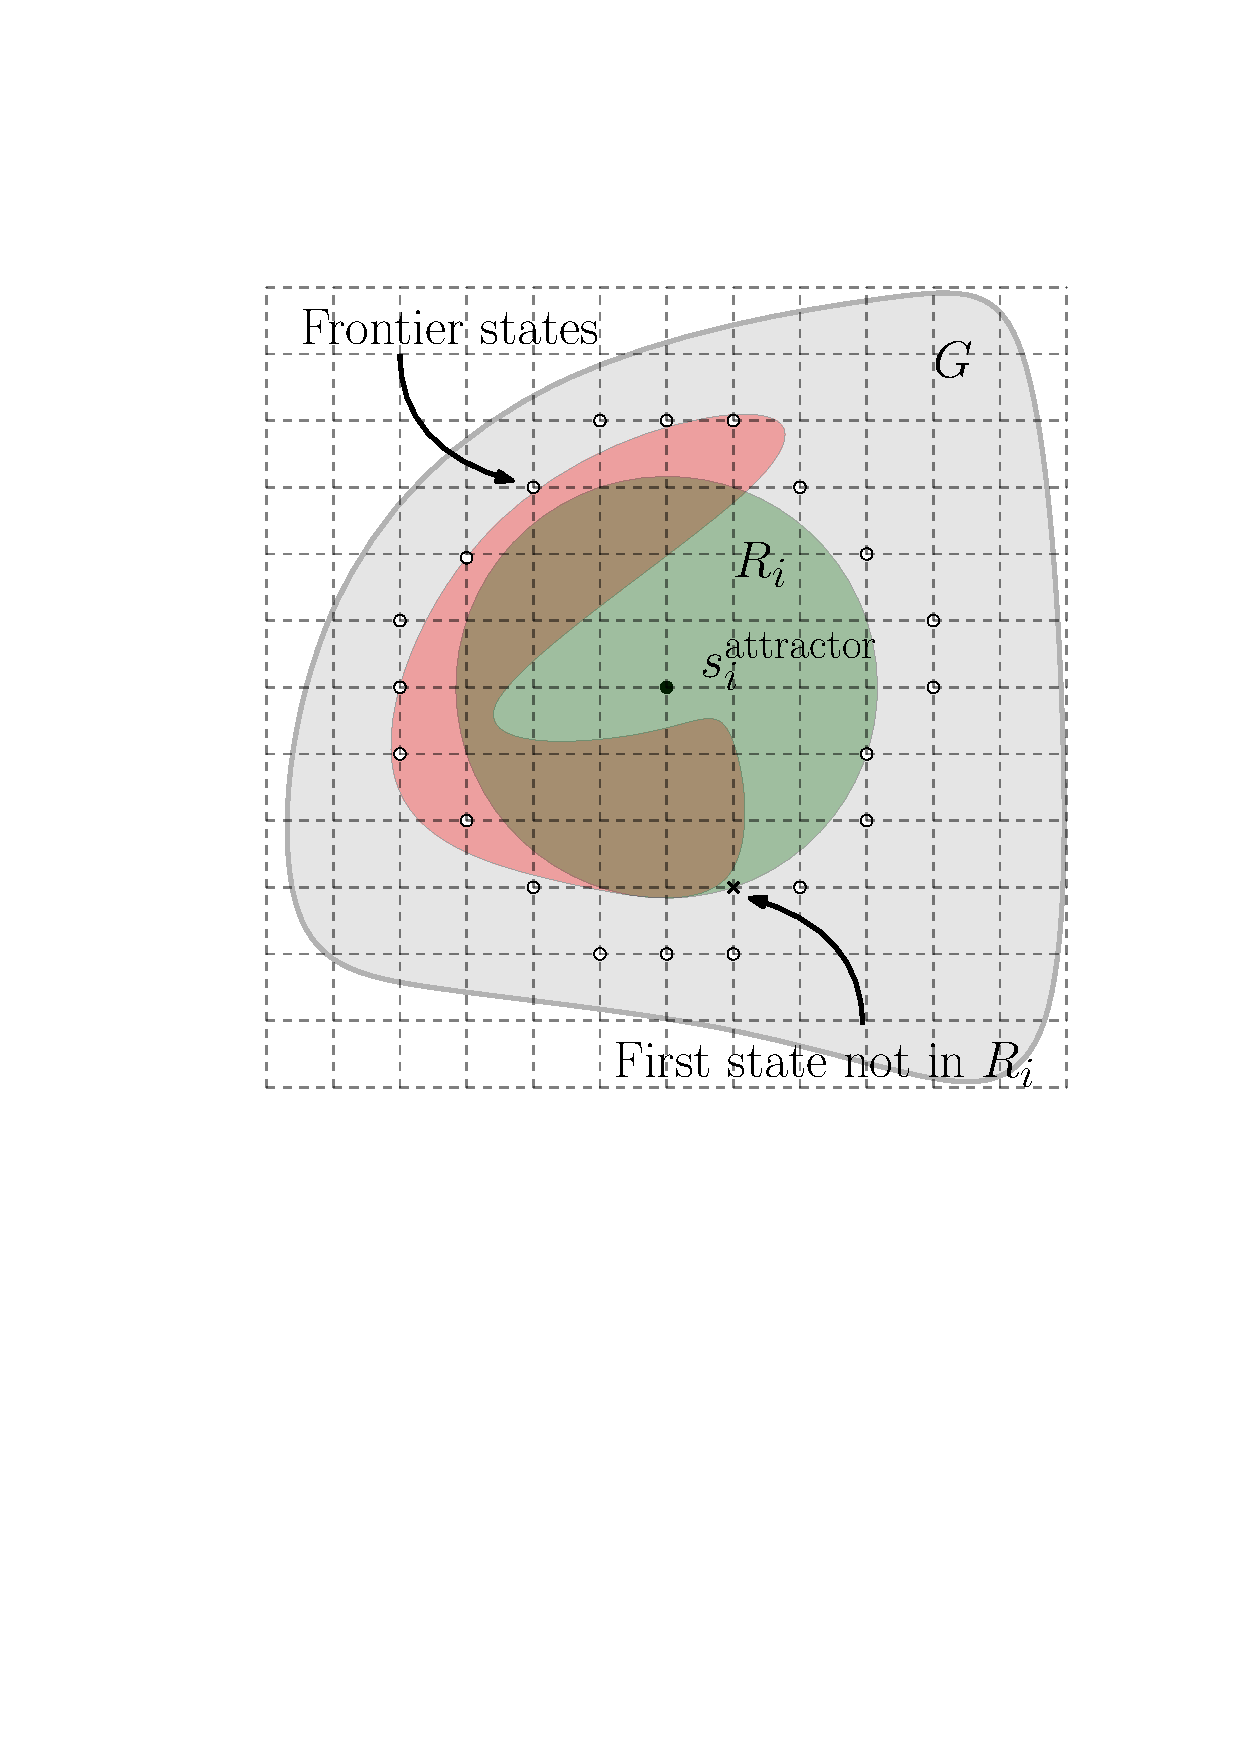
\includegraphics[width=0.25\textwidth]{Alg2.pdf}
  	% \vspace{-2mm}
  \caption{
  Visualization of Alg~\ref{alg:2}. Subregion $R_i$ (green) grown from $\sAttract$ in a goal region~$G$ (grey) containing an obstacle (red).
  Frontier states  and first state not in $R_i$ are depicted by circles and a cross, respectively.
}
   	\label{fig:alg2}
 \vspace{-5mm}
\end{figure}

\begin{table}[tb]
  \begin{center}
    \begin{tabular}{ l c c }
       & \textsf{PRM} & Our method \\ 
     \hline
     Mean Planning time [ms]& 6.84 	& 0.55 \\  
     Success rate [$\%$]	& 90 	& 100 \\
     Memory usage [Mb] 		& - 	& 0.2 \\
    \end{tabular}
    \caption{Experimental results comparing our method with \textsf{PRM}.}
    \label{tab:stats}
  \end{center}
%  \vspace{-3mm}
\end{table}

\paragraph*{Reachability Search}
The core of our planner lies in the way we compute the subregions (Alg.~\ref{alg:2} and Fig.~\ref{fig:alg2}) which we call a ``Reachability Search''. The algorithm maintains a set of \emph{reachable} states $S_{\text{reachable}}$ for which property P1 holds. 
Namely, the greedy successor\footnote{A state $s' \in \text{Succ}(s)$ is said to be a \emph{greedy} successor according to some heuristic $h(\cdot)$ if it has the minimal $h$-value  among all successors.} $s'$ of every reachable state $s \in S_{\text{reachable}}$ is also a reachable state, except for the attractor state \sAttract. 
This will ensure that in the query phase, we can run a greedy search from any reachable state $s \in S_{\text{reachable}}$ and it will terminate in the attractor state. 

The algorithm computes a subregion that covers the maximum number of reachable states that can fit into a hyper-ball defined by $h(s,\sAttract)$. 
The search maintains a priority queue OPEN ordered according to $h(s,\sAttract)$. Initially, the predecessors of $\sAttract$ are inserted in the OPEN (line~\ref{alg:2:OPEN}). For each expanded predecessor, if its valid greedy successor is in $S_{\text{reachable}}$, then the predecessor is also labeled as reachable (lines~\ref{alg:2:crit} and~\ref{alg:2:set}). 
%As the priority used for OPEN is the heuristic function, the radius of this hyper-ball keeps on increasing (line~\ref{alg:2:rad}). 


The algorithm terminates when the search pops a state which is valid but does not have a successor state in $S_{\text{reachable}}$ (line~\ref{alg:2:terminate}). Intuitively, this corresponds to the condition when the reachability search exists an obstacle (see Fig.~\ref{fig:alg2}). At termination, all the states within the boundary of radius $r_i$ (excluding the boundary) are reachable.


\begin{algorithm}[t]
\footnotesize
\caption{Reachability Search}\label{alg:2}

\begin{algorithmic}[1]
\Procedure{ComputeReachability}{$\sAttract$}
%\Procedure{ComputeReachability}{$\sAttract, r_{\text{max}}$}
\State $S_{\text{reachable}} \leftarrow \{\sAttract\}$ \Comment{Reachable set} \label{alg:2:reachable}
\State OPEN $\leftarrow \{$Preds($\sAttract$)$\}$  \Comment{key: $h(s,\sAttract)$} \label{alg:2:OPEN}
\State $r_i \leftarrow 0$

%\While {$r_i \leq r_{\text{max}}$}
\Loop{}
    \State $s \leftarrow$ OPEN.pop()
    \State $s'_g \leftarrow \arg \min_{s' \in \text{Succ}(s)} h(s', \sAttract)$ 
%    \State $s'_g \leftarrow$ GreedySucc($s$) 
 \Comment{greedy succesor}
 % acc. to some tie-breaking criteria}
    \If {$s'_g$ $\in$ $S_{\text{reachable}}$ and Valid(edge(s,$s'_g$))}  \label{alg:2:crit}
        \State $S_{\text{reachable}} \leftarrow S_{\text{reachable}} \cup \{s\}$  \Comment{$s$ is greedy} \label{alg:2:set}
    \ElsIf {Valid($s$)} \label{alg:2:terminate}
		\State \Return $r_i$
%        \State break
    \EndIf
    \State $r_i \leftarrow h(s, \sAttract)$ \label{alg:2:rad}
    \For {each $p \in \text{Preds}(s)$}
        \If {$p \notin S_{\text{reachable}}$}    \Comment{avoid re-evaluation}
            \State Insert $p$ in OPEN with priority $h(p, \sAttract)$
        \EndIf
    \EndFor
\EndLoop
%\EndWhile
%\State \Return $r_i$

\EndProcedure
\end{algorithmic}
\end{algorithm}

\subsubsection{Query Phase}
For any query goal state $s_{\text{goal}} \in G$, we find a subregion $R_i \in \calR$ which covers it. Namely, a region~$R_i$ for which 
$h(s_{\text{goal}}, \sAttract) < r_i$.
We then run a greedy search starting from $s_{\text{goal}}$ by iteratively finding for each state $s$ the successor with the minimum heuristic $h(s, \sAttract)$ value until the search reaches \sAttract. The traced path is then stitched to the corresponding precomputed path~$\pi_i \in \calL$. 
Note that at no point  do we need to perform collision checking in the query phase.

The query time comprises of 
(i)~finding the containing subregion $R_i$ 
and
(ii)~running the greedy search to $\sAttract$.
Step (i) requires iterating over all subregions which takes $O(|\calR|)$ steps while 
step (ii) requires expanding a number of states which is proportional to $r_i$.
Thus, after the preprocessing stage the maximal query time can be computed.




% which makes the query phase highly efficient.

%\subsection {Theoretical Properties and Computational complexity}
%TODO

\section{Evaluation}
We evaluated our algorithm on a PR2 for the single-arm (7 DOF) planning problem depicted in Fig.~\ref{fig:sim}. The task here is to repeatedly pick up objects from a conveyor belt and put them in a bin. 
We define the task-relevant goal region~$G$ by bounding the position and orientation of the end effector. 

%As mentioned, our method allows to guarantee bounds on the query time. The worst-case query time is bounded using the radius of the largest subregion and the total number of subregions that cover $G$. 
%After the preprocessing stage we can compute it by adding the lookup time for iterating over all the regions, and the time that the greedy search takes to reach the attractor from a goal state lying on the boundary of the largest subregion.

%\subsection{Results}
We compared our approach with the \textsf{PRM} algorithm in terms of success rate and planning times (see Table~\ref{tab:stats}) for 100 uniformly sampled goal states from $G$. 
Preprocessing (Alg.~\ref{alg:1}) took 950 seconds and returned 898 subregions. For a fair comparision the \textsf{PRM} was given the same amount of preprocessing time and the paths from all the nodes in $G$ to $s_{\text{start}}$ were precomputed. 
In the query phase if \textsf{PRM}'s connect operation fails for a given query, we consider it a failure. 
We also bootstrap \textsf{PRM} with 20 goal states from $G$. 


\begin{figure}[tb]
  \centering
    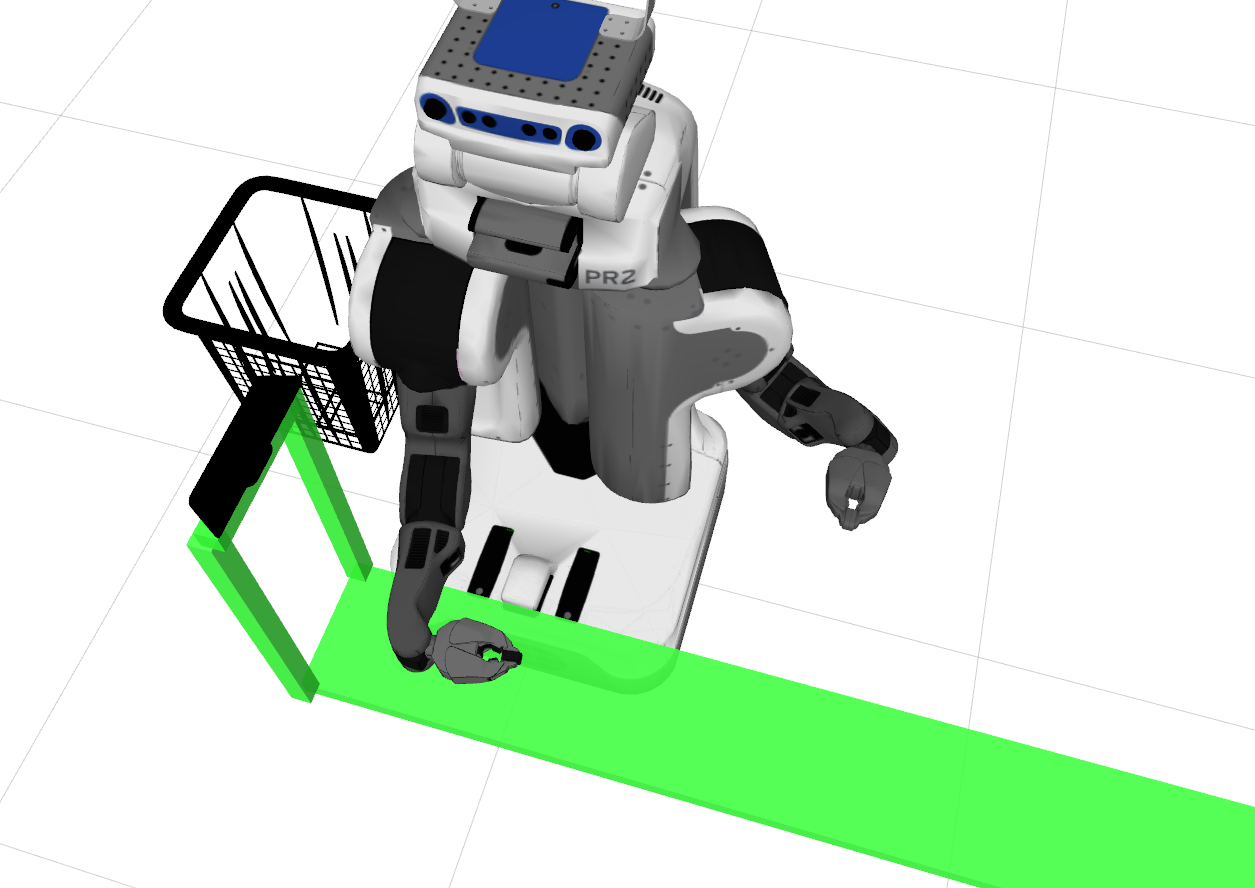
\includegraphics[width=0.325\textwidth]{simulation2.png}
    % \vspace{-2mm}
  \caption{
  Experimental setup.
}
    \label{fig:sim}
 \vspace{-3mm}
\end{figure}



%\section{Conclusion}
%Proofs
%
%Computational complexity

%%%%%%%%%%%%%%%%%%%%%%%%%%%%%%%%%%%%%%%%%%%%%%%%%%%%%%%%%%%%%%%%%%%%%%%%%%%%%%%%
\bibliographystyle{plain}
\bibliography{references}

\end{document}
